\documentclass{article}
% Choose a conveniently small page size
% PACKAGES
\usepackage[margin = 1in]{geometry}
\usepackage{amsfonts}
\usepackage{amsmath}
\usepackage{amssymb}
\usepackage{multicol}
\usepackage{graphicx}
\usepackage{float}
\usepackage{xcolor}
\usepackage{amsthm}
\usepackage{dsfont}
\usepackage{hyperref}

% MACROS
% Set Theory
\def\N{\mathbb{N}}
\def\R{\mathbb{R}}
\def\C{\mathbb{C}}
\def\Z{\mathbb{Z}}
%\def\^{\hat}
\def\-{\vec}
\def\d{\partial}
\def\!{\boldsymbol}
\def\X{\times}
%\def\-{\bar}
\def\bf{\textbf}
\def\l{\left}
\def\r{\right}
\title{Report: November 27, 2023}
\author{Damien}
\begin{document}
\maketitle
% \newpage
\section{Progress}
I have the algorithm working. I realized that one needs to average the upwind and downwind fluxes on both the forward and backward sweeps. 
\begin{figure*}[h]
    \centering
    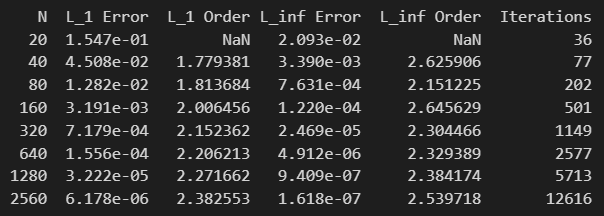
\includegraphics[width=0.5\textwidth]{imgs/table.png}
    \caption{This plot is an attempt to reproduce the results from Table 1 in Chen et al.}
    \label{fig:grid}
\end{figure*}
This table is not exactly the same as the results from the paper. However, it clearly shows a fast rate of convergence between second and third order accuracy. I have a few ideas as to why I am not quite achieving the expected accuracy. They have to do with the convergence conditions and how I choose the number of points. I am rather certain that the implementation itself is solid.
\section{To Do}
For next week I will try to figure out why this plot is different from what is in the paper, improve the performance of the code because it runs rather slowly, and implement the solution to 5.3.1 in Chen et al.
\end{document}